\chapter{Event Reconstruction}
\label{chap:eventreco}

\section{Basic Elements From the Detector} 

Depending on their nature, the particles emanating from the collision leave various forms of energy deposits in the different subdetectors. All these signals need to be aggregated and processed to allow for the reconstruction of what could be considered particle-level information. The first step in this process consists of building \textit{Particle Flow elements} using information only locally within each subdetector. There are four primary elements from the subdetectors: tracks from the tracker, calorimeter deposits in each the ECAL and HCAL, and tracks from the muon detector. As will be discussed in the next section the elements are combined via the Particle Flow \textit{algorithm}, yielding reconstructed particles used for physics analysis.

Note that the definition of any object within the detector makes use of additional selection criteria which is not generally discussed here. For instance, one may require that a track in the tracker have at least 3 hits in the pixel detector, or that a calorimeter hit is above some minimum threshold energy. The effects of this selection is generally a balance between the reconstruction efficiency of any given particle and the probability to misidentify a particle (purity).

This chapter is adapted from \cite{CMS-PRF-14-001}.

\subsection{Tracks and Vertices}

Tracker hits are formed in the pixel and strips detectors by clustering any hits in neighboring elements of the detector plane. The cluster position is measured by weighted sums of the individual channel positions. Charge sharing among detector channels allow for a finer spatial resolution in the position measurement. Track reconstruction first begins by forming track seeds consisting of a small number of detector hits. These track seeds are then projected onto successive detector layers looking for nearby additional hits. This follows the Kalman filtering procedure, in which track information is updated after the addition of each hit. Electron tracking is performed with a slightly modified algorithm to better account for the energy loss mechanisms as the electron traverses the detector. \cite{trackerreco}

The track building procedure follows an iterative procedure, where the requirements on the quality of the track seed decrease as the iterations proceed. The first iterations begin with seeds consisting of 3 pixel hits and lead to high performance reconstruction of high $p_{T}$ tracks emanating from the collision region. The iterations proceed until essentially only requiring hits in the outer tracker and reconstructs displaced tracks or those missing hits. The iteration procedure provides a balance between reconstruction efficiency, track purity, and computation economics. Table \ref{tab:itertracks} list these iterations - the requirements on the seed and types of tracks that iteration targets.

\begin{table}[h]
\caption{Iterative tracking steps.\cite{CMS-PRF-14-001}}
\centering
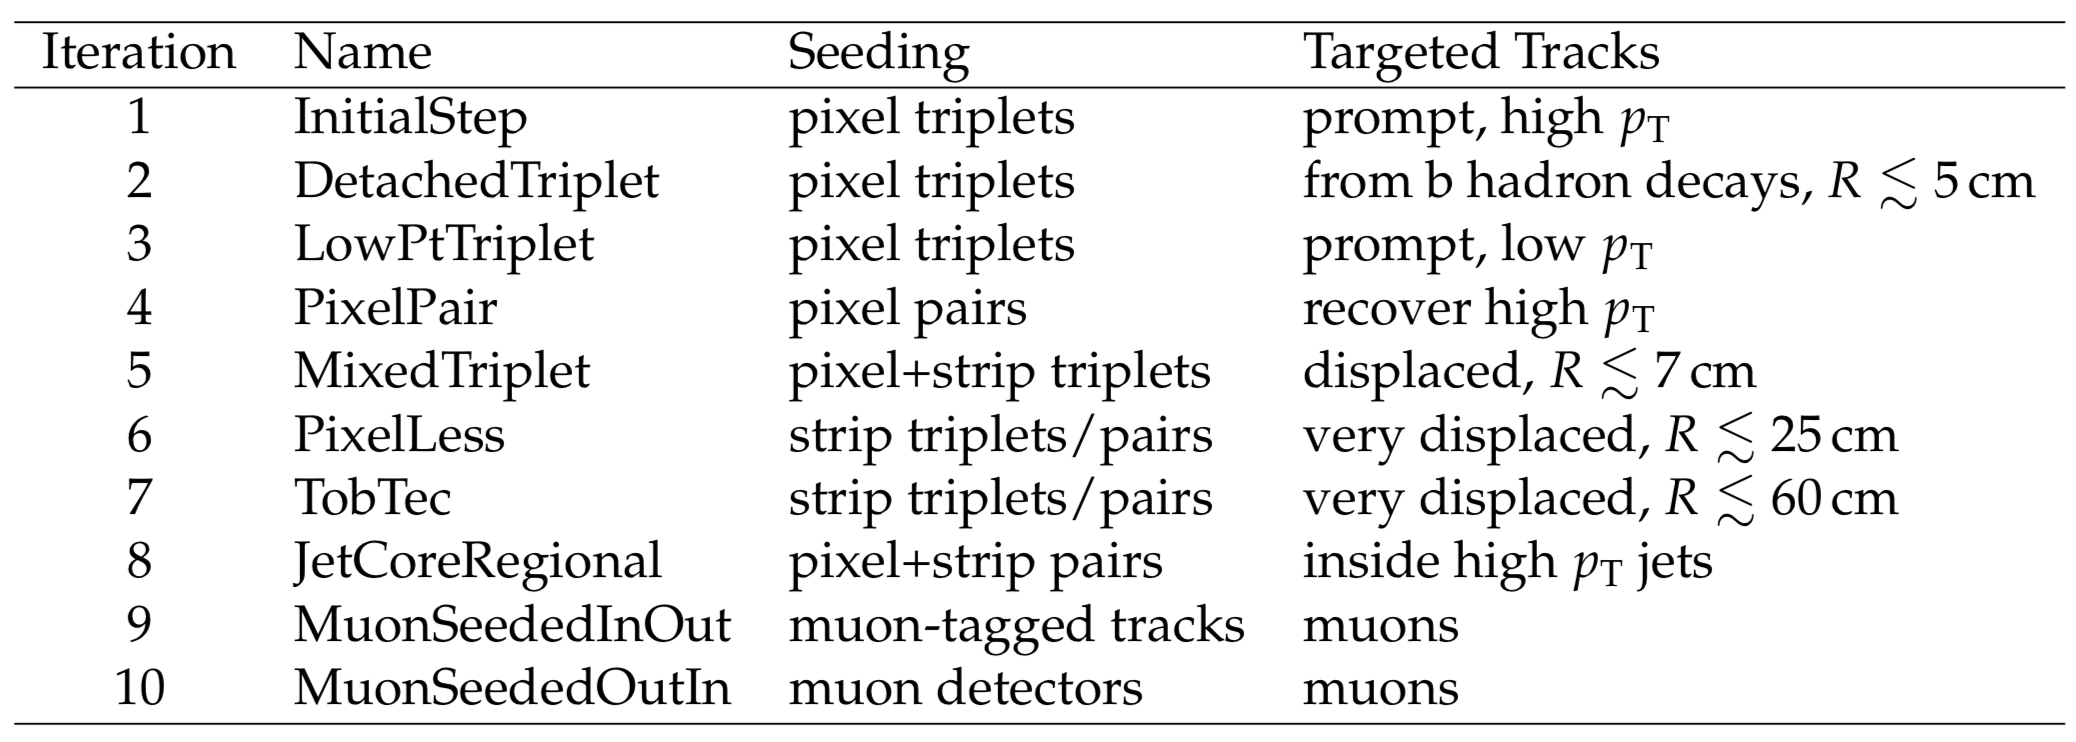
\includegraphics[width=0.8\textwidth]{figs/itertracks.png}
\label{tab:itertracks}
\end{table}

\subsection{ECAL \& HCAL Clusters}

\textit{Superclusters} are built by first identifying a crystal with the largest energy deposit, this is called a \textit{seed}. The supercluster is then formed by aggregating any hits among the neighbors (8) of the hits already in the cluster. This process then proceeds building all the superclusters and consuming all the calorimeter hits. Superclusters are built separately in the barrel and endcap. Within a given supercluster, N clusters are identified using an iterative algorithm assuming the observed hits arise from N Gaussian-distributed energy deposits; each of energy E, position in the $\eta-\phi$ plane $\vec{\mu}$, and width $\sigma$ scale set by the crystal size.

\subsection{Muon Tracks}

As there are multiple detector layers within a single muon station, track segments are locally formed within a chamber for both the DTs and CSC. These track segments represent the muon momentum at that station; pattern recognition is able to provide to measurement and its high speed allows the segments to be used trigger primitives for the muon systems, as was seen in Figure \ref{fig:trigger}. For track reconstruction, the track segments act as seeds for the track finding algorithm. The hits in each the DT, CSC, and RPC subdetectors are used in the final track reconstruction.

The geometry of the DT system allows for up to 32 measurements of the r-$\phi$ position and 16 for the r-z. The geometry of the CSC system allows for any in between 20-28 hits, depending on the position $\eta$. The geometry of the RPC system allows for any in between 6-10 hits, depending on the position $\eta$. 

\section{Obtaining a Particle-level Description}

Once the elements have been built, the Particle Flow algorithm exploits the information from each of the detectors to form the best possible particle candidate. \cite{CMS-PRF-14-001}. As different varieties of particles have unique signatures in the detector, particle identification is aided by the particular combination of elements \textit{linked} with one another. An illustrative example of these combinations we have seen in Figure \ref{fig:schematicview}  Elements are linked when projections from one element to the other are spatially consistent. There are four primary links:

\begin{itemize}
\item Tracks formed in the tracker are linked to an ECAL or HCAL cluster if the projection of the track, at a depth of the expected maximum of a shower in the ECAL or at one interaction length inside the HCAL, lies within the cluster area.
\item ECAL and HCAL clusters are linked if the ECAL cluster falls within the envelope of the HCAL cluster; ECAL provides finer spatial resolution compared to the HCAL.
\item A tracker track and a muon track are linked if their projections onto a common surface are spatially consistent.
\item To collect bremstrahllung radiation (photons) associated to an electron track, an ECAL cluster is linked to tracker tracks if projections tangent to the track at any of the tracker layers lies within the cluster volume. Additionally, as the probability for a photon to convert to an $e^{+}e^{-}$ pair is significant (XX\%) within the tracker, track pairs are linked if they are consistent with photon conversion.
\item If a Preshower cluster is within the envelope of an ECAL cluster the two are linked; Preshower has finer spatial granularity.
\item Tracks consistent with arising from a secondary vertex are linked to allow for reconstruction of nuclear-interactions.
\end{itemize}

Particle Flow \textit{blocks} are constructed by aggregating objects directly or indirectly linked with one another. The Particle Flow algorithm then processes each block in turn to create the final reconstructed particles. The algorithm builds the objects in the following order

\begin{enumerate}
\item \textbf{Muons}:
There are three types of tracks which can be used for muon reconstruction:
\begin{itemize}
\item
\textit{\textbf{standalone}} muons are built from tracks reconstructed solely in the muon system.
\item
\textit{\textbf{tracker}} muons are built from tracks reconstructed solely in the inner silicon tracker. It is tagged as being from a muon if, when projected onto a common surface, it is spatially consistent with a muon solely reconstructed from the muon chambers. Tracker muons have the best resolution for muons up to a $p_{T}$ of 200 GeV, as these are more likely to suffer from multiple scattering before enter the muon chambers.
\item
\textit{\textbf{global}} muons are reconstructed using the hits from both the inner silicon tracker and the muon stations.  The track pairing is the same done for tracker muons. For momenta above 200 GeV, the use of the muon system for tracks improves the momentum measurement.
\end{itemize}

Any ECAL or HCAL clusters associated with the muon track are used as muon selection/definition criteria if those clusters are found to be consistent with the muon hypothesis.

\item \textbf{Electrons \& Isolated Photons}:

An electron is formed by combining a track in the silicon tracker with a cluster in the ECAL. Its energy assignment uses a combination of both elements. The momentum direction is made using the track in the silicon tracker, as it gives greater spatial resolution.  A photon is defined as an ECAL cluster not associated with a track. Photon isolation is a requirement on the sum of the track $p_{T}$ within a cone $\Delta R = 0.3$around the photon; photons which arise during hadron fragmentation (i.e. poor isolation) are treated in the next section. 

Electrons and isolated photons are reconstructed within the same Particle Flow step to account for similar behavior within the tracker bulk. There is a large probability for both a) an electron to radiate a brehmsstrahlung photon and b) for a photon to convert to an e$^{+}$e$^{-}$ pair. Therefore in object reconstruction care must be taken to collect the photons radiated from electrons in order to make appropriate measurements of the particles.

\item \textbf{Hadrons \& non-isolated Photons}:

Hadrons \& non-isolated photons result from hadronization/fragmentation of jets. ECAL clusters not associated to any tracks are assigned to be photons. Neutral hadrons ($K^{0}_{L}$, neutrons) are reconstructed from HCAL clusters with no associated track; neutral hadrons leave a very small amount of energy in the ECAL. Charged hadrons ($\pi^{\pm}$, K$^{\pm}$, protons) are reconstructed using the remaining tracks and HCAL deposits. Charged hadrons do not radiate bremsstrahlung photons nor cause $e^{+}e^{-}$ pair creation and thus do not leave signals in the ECAL.

\item \textbf{Nuclear Interactions}:

Nuclear interactions often occur when outgoing particles interact within the detector material causing a shower of secondary particles. If multiple tracks are linked through a common secondary vertex they will be be summed to create a single charged hadron particle which replaces its constituents in the particle list of the event.

\end{enumerate}

\section{Additional High-Level Objects}

\subsection{Jets}

Bare quarks and gluons can never be observed in Nature due to a QCD phenomenon called \textit{color confinement}. Therefore, quark and gluon production manifests as a ``jet'' of color-neutral particles emanating from the production point. These particles can be clustered together to reconstruct the original parton. The jets used in this analysis are made by clustering particles with the ``anti-kt`` algorithm with cone sizes of $\Delta R$ = 0.4, 0.8 \cite{1126-6708-2008-04-063}, denoted as AK4 and AK8 jets respectively. This algorithm produces nearly conical jets but with an added benefit of being more robust to effects of soft radiation. The AK4 jets subtend less solid angle and are used to capture the hadronisation of single quarks and gluons. AK8 jets subtend a larger solid angle and are used for reconstruction of boosted objects (e.g. $t$, H, Z, W).

\subsection{b-tagging of Jets}

Jets resulting from the production of b quarks (and to some extent c quarks) garner special attention in our experiment. As usual for quarks and gluons, the b-quark will quickly hadronize and form a b hadron. But what is unique about the b hadrons are the values their lifetimes take such that they can travel hundreds of $\mu$m before decaying inside our detector. Vertexing the tracks resulting from the decay will reveal the presence of a \textit{secondary vertex} which is spatially displaced from the rest of the hadrons inside the jet. This secondary vertex allows for one handle on being able to identify jets as coming from b quark production. Other handles include the momenta and multiplicity of the other particles clustered into the jet.

In addition to tagging jets as originating from a single b quark, tagging of jets as originating from \textbf{two} b quarks is also possible.\cite{bbtagger} As would be expected, this technique makes heavy use of the presence of \textbf{two} secondary vertices. The analysis presented in Section \ref{chap:analysis} makes extensive use of this technique.

\subsection{Neutrinos -- Invisible Particles $\rightarrow p_{T}^{\mathrm{miss}}$}

Neutrinos are so weakly interacting that they leave no energy deposits in CMS and therefore cannot be detected by our experiment. Although direct detection is not possible, we are still able to \textit{infer} the presence of a neutrino. The protons involved in the initial collision have no net momentum in the transverse direction; the summed momenta of all the final state particles should therefore be equal to zero in the direction transverse to the beamline. Any non-zero value for the final-state transverse momentum is thus indicative of a neutrino escaping unscathed. We define this imbalance as:

\begin{equation}
p_{T}^{\mathrm{miss}}  \equiv \left | - \sum_{i} \vec{p_{T}} \right |,~\forall~\textrm{particles~i}.
\end{equation}

In addition to SM neutrinos, many theories of beyond the Standard Model physics predict particles which are expected to give rise to a source of $p_{T}^{\mathrm{miss}}$ as they (presumably) would not interact with our detector.

\subsection{$\pi^{0}$ meson}

Charged and neutral $\pi$ mesons are the lightest of all hadrons with masses of 135 and 140 MeV, respectively. The next massive are the K mesons at ~495 MeV; the lightest baryons are neutrons and protons, with masses of 940 MeV. Pions are therefore copiously produced within hadronic interactions and often contain much of the jet energy. As a rule-of-thumb, the charged to neutral energy fraction within a jet is approximately two-thirds to one-third (to match the pion and Kaon multiplicities).

Because the neutral pion branching to photons is over 98\% and its lifetime is relatively short (25.5$\,$nm), the detection of neutral pions therefore involves reconstruction of photon pairs with the appropriate invariant mass. This is simple enough in principle, but as the pion $p_{T}$ increases the photons from the pion decay become more and more collimated. Eventually, for pions above about 7 GeV, individual photons are not able to be resolved because of the ECAL resolution (crystal size), the same crystal gets the energy from both photons. This was the primary motivation for the Preshower ECAL detector.
